\documentclass[12pt,A4]{book}
\title{MIDILC:  A MIDI Language Compiler for Programmatic Music Composition}
\author{Alex ``Akiva'' Bamberger \\ Benjamin Mann \\ Fredric Lowenthal \\ Ye Liu}
\date{}

\usepackage{graphicx}
\usepackage[margin=1in]{geometry}
\begin{document}
\maketitle
\newpage
\tableofcontents
\newpage
%commit
\chapter{Introduction}
The language, hereafter referred to as MIDILC (pronounced MIDDLE C, standing for MIDI
Language Compiler), allows programmers to compose music. It compiles into MIDI format and
has syntax that is similar to Java, changing the basic primitives and the meaning of various
operators (Fig \ref{fig:types_in_midilc}).
% TODO the figure says nothing about operators...
\begin{figure}
\center
\begin{tabular}{|p{.2\textwidth}|p{.5\textwidth}|}
\hline
\verb|Number| & a value between $-2^{31}$ and $2^{31}-1$\\ \hline
\verb|Note| & a musical note with pitch and duration \\ \hline
\verb|Chord| & stores notes with equal durations and start times, represented by an integer list \\ \hline
\verb|Sequence| & a sequence of notes and chords, represented by a list of integer lists \\ \hline
\end{tabular}
\caption{Types in the MIDILC language. }
\label{fig:types_in_midilc}
\end{figure}

The langauge is dynamically typed, but introduces preset types for the programmer most comfortable with the syntax of C or Java. Types must be used upon variable declaration, but are left optional for function declarations and arguments. Each type can be safely cast up in the following order: \verb|Number| $\rightarrow$ \verb|Note| $\rightarrow$ \verb|Chord| $\rightarrow$ \verb|Sequence|. The standard library, written in the language itself, supports major and minor chords, arpeggios, repetition, and other such basic and often used concepts. Note durations are specified in terms of whole notes (w), halves (h), quarters (q), eigths (e), and sixteenths (s). Sequences can either be appended to, which advances the ``current time'' by however long the appended sequence is, or else something can be inserted into a sequence at a given offset using subscripting. Functions are specified in the same way as in C.

Sequences and Chords can be output to the intermediate representation (IR) of CSV format using the play() function. In order to actually write the MIDI files, the CSV is fed to a Java program that interprets the CSV using the javax.sound.MIDI package.

Composing music on a computer is often done using GUIs that allow the user to drag and drop notes or using instrument inputs. This lets the musician hear his compositions as he is creating them, and often gives the musician a simple MP3 or MIDI ouput. As computer scientists, the MIDILC team finds such methods tedious, extraneuous and requiring too much natural music talent. MIDILC appeals to the virtues of any great programmer: laziness, hubris, and impatience \footnote{Wall, Larry. \textit{Programming Perl}, O'Reilly 2000.} and propose a language for those wishing to turn their quantitative skills into beautiful music.

MIDILC also attempts to redress other issues of regular music composition. Songs often have frequent recurring themes. Manually reusing these themes requires precision and dedication. If pieces of a song could be manipulated automatically for reuse and slight modification, song production speed could increase dramatically. The MIDILC language allows programmers to algorithmically generate notes, chords, and sequences of notes and chords by writing functions. This allows for writing interesting compositions that minimize time spent rewriting basic MIDI manipulation routines and implementing primitive musical constructs. The language works optimally with compositions that make consistent use of simple motifs as it encourages reuse of simple mathematical operations on notes and chords. 

MIDILC is tailored for crafting melody sequences. For a sequence containing a series of whole notes, one could easily manipulate the notes in the melody to create sequences of counterpoints to the melody. Using MIDILC, a \verb|major()| and \verb|minor()| function are easy to craft and chords simple to arpeggiate to make counterpoint. MIDILC allows for the simple concatenation and composition of sequences, and so complicated sequences could be easily made from simple starting blocks.

\chapter{Language Tutorial}
MIDILC was designed with the programmer in mind, but uses all the musical notation familiar to the musician. The lanuage is robust enough to fully support the idiomatic construction of Notes and Chords, as well as set tempo and note duration using \verb|Note| and \verb|Number| literals.
\section{An Introduction}
MIDILC is a C-like language used for generating midi music algorithmically. Each source file, with the extension .m, should contain a main() method. Like C, each line of code should be terminated with the semicolon.
\begin{verbatim}
main() {
    some_function();
\end{verbatim}

MIDILC’s basic types are Number, Note, Chord, and Sequence, the last three of which can be written into .midi files and played. All variables must be declared, one at a time, before they are called.

% TODO this is wrong

\noindent Numbers, the most basic type in MIDILC, supports integer values from 0 to 127. These numbers correspond to the 128 MIDI instruments and notes.

\vspace{5 mm}

\verb|Number num;| /*declares the variable num */

\verb|num = 4;| /* sets num to 4 */

\verb|num = num + 1;| /* increment num by 1, so that it is now the value 5 */

\vspace{5 mm}

\noindent The following snippet will provide you with a Note, the simplest of the playable musical types.

\vspace{5 mm}

\verb|Note n;| /* declares the variable n*/

\verb|n = A;| /* sets n to the note A, which by default is in 

\indent \indent \indent the 3rd octave and a quarter note */

\vspace{5 mm}

\noindent Notes can also be initiated with more options:

\vspace{5 mm}

\verb|n = A4w;| /* sets n to the note A, in the 4th octave, as a whole note */

\verb|n = A4w + 4;| /* sets n to A in the 4th octave as a whole note, 

\indent \indent \indent and add 4 beats (a quarter note’s worth) to its duration */

\verb|n = A4w .+ 4;| /* sets n to A in the 4th octave as a whole note, then 

\indent \indent \indent increase its pitch by 4 half steps (to C sharp) */

\vspace{5 mm}

\noindent The next type, \verb|Chord|, can be constructed from scratch, or based on notes that already exist. Unlike Note, Chord objects must be initiated with the \verb|new_chord()| function. Notice that since the \verb|+=| operator is not supported, adding to a \verb|Chord| requires one to set the Chord to itself plus the added object.

\vspace{5 mm}

\verb|Chord a;|

\verb|Chord b;|

\verb|Chord c;|

\verb|Chord d;|

\verb|a = new_chord();| /* initializes a Chord object that plays nothing */

\verb|b = new_chord(C, E, G);| /* initializes b to be a C major chord in the 

\indent \indent \indent (default) 3rd octave with (default) duration of a quarter note*/

\verb|c = new_chord(n);| /* initializes c to be a chord containing Note n */

\verb|a = a + n;| /* adds the note n to a, which previously contained nothing playable */

\vspace{5 mm}

\noindent Sequence objects can be thought of as a collection of Note, Chord, and other Sequence objects. Construction of new Sequence objects is similar to that of new Chord objects. Both Note and Chord objects can be added to a Sequence object, in any permutation.

\vspace{5 mm}

\verb|Sequence s1;| /* declares s1 */

\verb|Sequence s2;| /* declares s2 */

\verb|s1 = new_sequence();|  /* initializes s1; empty sequence */

\verb|s2 = new_sequence();|  /* initializes s2; empty sequence */

\verb|s1 = s1 + C4e;| /* adds a note to s1 (4th octave C, eighth note duration) */

\verb|s1 = s1 + R;| /* adds a rest to s1 */

\verb|s2 = s2 + a;| /* adds Chord object a to s2 */

\verb|s2 = s2 + b;| /* adds Chord object b to s2 */

\vspace{5 mm}

\noindent Finally, to print Sequence objects to .midi, the \verb|play()|function is invoked. \verb|play()| takes as an argument a \verb|Sequence| to be written out, and each time \verb|play()| is called, a new track is created. Thus, multiple calls of \verb|play()| in the same file will result in a multi-track .midi being created.

\vspace{5 mm}

\verb|play(s1);| /* prints s1 out as a track */

\verb|play(s2);| /* prints s2 out as a second track */

\vspace{5 mm}

\noindent MIDILC does not give the user the responsibility of memory management. Therefore, to complete a basic program using the code snippets above, simply close the \verb|main()| function with the corresponding bracket.

To compile the program that you have just written, type the following into the command line:

\vspace{5 mm}

\verb|./midilcc sample_program.m [sample_program_output]|

\vspace{5 mm}

\noindent The last parameter is optional; if not given, a default name consisting of the name of the .m file with a .csv extenion will be given to the output CSV file. The compiler will print out any errors that may have occurred, and if the compilation was successful, a .csv file and a .midi file will be created in the same directory as the .m file. Simply open the .midi file with any media player to play it.
\section{Twinkle Twinkle Little Star}

\indent The following tutorial will guide you through a simple program written in MIDILC, which produces a .midi file of the familiar tune “Twinkle Twinkle Little Star”. The full code can be found in the appendix.
	
The source files of MIDILC are saved as .m text files. First, create a .m file; call it twinkle.m. We 
will have one function, namely the \verb|main()| function, for all the code in this program. We declare the 
\verb|main()| function, and declare all the variables used, one per line:	

\vspace{5 mm}

	/* twinkle twinkle little star*/

\verb|main() {|

		/* declare all the variables: Notes c through a, Sequences
		first part and overall, and Number n */

\verb|Note c;|

\verb|Note d;|

\verb|Note e;|

\verb|Note f;|

\verb|Note g;|

\verb|Note a;|

\verb|Sequence firstpart;|

\verb|Sequence overall;|

\verb|Number n;|

\vspace{5 mm}

\noindent The next step is to initialize all the variables. We will start with the \verb|Note| objects.

\vspace{5 mm}

/* set each of the notes to a quarter note in the 4th octave, note name as 
indicated by the capital letters */

	\verb|c = C4q;| /* note C, in the 4th octave, quarter-note duration */
	
	\verb|d = D4q;|
	
	\verb|e = E4q;|
	
	\verb|f = F4q;|
	
	\verb|g = G4q;|
	
	\verb|a = A4q;|

\vspace{5 mm}

\noindent Next, we initialize the \verb|Sequence| objects. Notice that unlike \verb|Note|, we must call on the new_sequence() function.

\vspace{5 mm}

	/* initialize sequences */
	
	\verb|firstpart = new_sequence();|
	
	\verb|overall = new_sequence();|

\vspace{5 mm}

\noindent Now, we are ready to add notes to the \verb|Sequence| objects. Let’s start with 
firstpart, which we will use to store the first two stanzas of the song.

\vspace{5 mm}

	/* add the first two stanzas of the song to 
	
	the \verb|Sequence| firstpart */
	
	\verb|firstpart = firstpart + c;|
	
	\verb|firstpart = firstpart + c;|
	
	\verb|firstpart = firstpart + g;|
	
	\verb|firstpart = firstpart + g;|
	
	\verb|firstpart = firstpart + a;|
	
	\verb|firstpart = firstpart + a;|
	
	/* make the last note's duration two quarter notes long 
	
	(4 beats longer, 16th note per beat) */
	
	\verb|firstpart = firstpart + (g + 4);|
	
	\vspace{3 mm}
		
	\verb|firstpart = firstpart + f;|
	
	\verb|firstpart = firstpart + f;|
	
	\verb|firstpart = firstpart + e;|
	
	\verb|firstpart = firstpart + e;|
	
	\verb|firstpart = firstpart + d;|
	
	\verb|firstpart = firstpart + d;|
	
	\verb|firstpart = firstpart + (c + 4);|
	
\vspace{5 mm}

\noindent Next, we will start building the main sequence (overall), using a loop 
for the middle two identical stanzas of the song.

\vspace{5 mm}

	/* add the first part to the overall \verb|Sequence| */
	
	\verb|overall = overall + firstpart;|
	
	\vspace{3 mm}
	
	/* add the middle section of the song to overall twice, 
by using a for-loop */

	
	\verb|for (n = 0; n < 2; n = n+1) {|
	
		\indent \verb|overall = overall + g;|
	
		\indent \verb|overall = overall + g;|
	
		\indent \verb|overall = overall + f;|
	
		\indent \verb|overall = overall + f;|
	
		\indent \verb|overall = overall + e;|
	
		\indent \verb|overall = overall + e;|
	
		\indent \verb|overall = overall + (d + 4);|
	
	\verb|}
	
	\vspace{3 mm}
	
	/* add firstpart to overall again, since they repeat*/
	
	\verb|overall = overall + firstpart;|
	
\vspace{5 mm}

\noindent We are almost ready to write the program out to a .csv file. Let us 
lower the tempo of the song from the default 120 beats per minute (bpm) 
to 90, then call on the play() function to create the CSV file.

\vspace{5 mm}

	/* set tempo from default 120 to 90, since it is a slow song */
	
	\verb|set_tempo(90);|
	
	/* call on play() to create the csv file */
	
	\verb|play(overall);|
	
\verb|}|

\vspace{5 mm}

\noindent Congratulations, you have just written your first MIDILC program! 
To compile the program, invoke the MIDILC compiler (midilcc), as 
described in the previous section.

\chapter{Language Reference Manual}

MIDILC is a C-like language that makes it simpler to algorithmically generate music.  It simplifies MIDI music creation by allowing programmers to specify song information in musical terms and write functions that process existing musical information.  By building off of simpler musical functions, such as arpeggios and chords, complex musical compositions can easily be programmed.

To eliminate the programming complexities from the MIDILC language, it has limited scope and data management capabilities.  MIDILC can be used following an imperative or functional paradigm and reduces hassle for the programmer by forcing static scope.

It compiles into MIDI files that can then be played in any standard media player.

\section{Lexical Conventions}
\begin{figure}
\center
\includegraphics[width=.75\textwidth]{notes.png}
\label{fig:pitches_and_notes}
\caption{The correspondence of notes and pitches in MIDI. }
\end{figure}
\subsection{Tokens}
Tokens consist of identifiers, keywords, constants, operators, and separators.  As with C, MIDILC is a free-form language and all white space characters are ignored (with the exception of separating tokens), as braces are used to identify the start and end of code blocks and semicolons are used to end statements.
\subsection{Comments}
/* and */ are used to indicate a block of comments (C-style comments).  There are no C++-style comments in MIDILC.
\subsection{Identifiers}
These are sequences of letters, digits, and underscores, starting with a letter or underscore.  Identifiers cannot be of the format \verb|[A-G R][b|\#\verb|]?[0-9]?[w h q e s]?|, as these are reserved for \verb|Note| literals.
\subsection{Keywords}
MIDILC has very few keywords; these include the following:

\begin{tabular}{|c|c|}
\hline
Types & Control \\ \hline
\verb|Number| & \verb|return| \\ \hline
\verb|Note|	& \verb|continue| \\ \hline
\verb|Chord| & \verb|break| \\ \hline
\verb|Sequence|	& \verb|if| \\ \hline
\verb|Void|	& \verb|else| \\ \hline
	& \verb|while| \\ \hline
	& \verb|for| \\ \hline
\end{tabular}


\subsection{Constants/Literals}
MIDILC allows a user to construct \verb|Note|s using pitch and duration (as \verb|Number| types), or using a set of \verb|Note| literals, specified by the note letter, accidental (if any), MIDI octave, and a letter that indicates the note’s duration (optional, and defaulting to a quarter note).  Duration can be specified by w (for whole note), h (for half note), q (for quarter note), e (for eigth note), and s (for sixteenth note).  Rests are indicated by using R instead of a note. Any \verb|Note| object constructed using a pitch with illegal properties will result in an error. \verb|Chord|s can easily be expressed using built-in chord generation function calls on \verb|Note| literals.  In addition, \verb|Number| literals also exist (integral numbers limited to signed 32-bit range).  MIDILC does not have floating-point literals.
Note that literals look like the following:
\verb|Ab7|,
\verb|C4s|,
\verb|G5h|

Pitches and \verb|Number| literals have the correspondence shown in figure \ref{fig:pitches_and_notes}.

\section{Meaning of Identifiers}
Identifiers in MIDILC have the following attributes: scope, name space, linkage, and storage duration. Since static scope is handled automatically, there are no storage class specifiers in MIDILC.
\subsection{Disambiguating Names}
\subsubsection{Scope}
The scope of of an identifier is defined as the region of a program within which it is visible, and begins when it is declared. In MIDILC, all identifiers are globally scoped, and are therefore visible to all blocks within a program unless hidden in another scope. This is due to the fact that the language automatically handles static identifiers.
\subsubsection{Name Space}
All the identifiers in MIDILC are categorized as ordinary identifiers. These include user-defined type names, object names, and function names.
\subsubsection{Linkage of Identifiers}
Identifiers in MIDILC may be linked across different files of the same program, but the identifier name must be unique in all files. Furthermore, the compiler will generate a compile time error about the identifier if there is a conflict.
\subsubsection{Storage Duration}
Storage duration denotes the lifetime of an object. All objects in MIDILC are static, and have static storage duration. The initialization of these objects occurs only once, prior to any reference.
\subsection{Object Types}
The MIDILC language supports two types of objects: numbers and musical notations.  Objects are dynamically typed.  Typing of an identifier is determined on assignment.
\subsubsection{Number type}
The only supported numerical type is \verb|Number|, which has a size of 32 bits and ranges from $-2^{31}$ to $2^{31} - 1$.  This is also the underlying type for all fields within the musical types.
\subsubsection{Musical types}
\verb|Note|, \verb|Chord|, and \verb|Sequence| are all of the musical types supported by MIDILC. \verb|Note| literals are  made up of strings consisting of integers and characters in sequences that match the following regular expression:
\verb|[A-G R][b |\#\verb|]?[0-9]?[w h q e s]?|
As these types are not stored directly internally, their sizes are not exact. As a general rule, for non-empty objects,
\verb|Number < Note < Chord < Sequence| in terms of their relative sizes.
\paragraph{Note type}
\verb|Note| type has the following attributes: pitch and duration. Pitch refers to the frequency of the note (Fig \ref{fig:pitches_and_notes}), and duration is specified as a type of note: whole, half, quarter, eighth, or sixteenth.  \verb|Note| literals with the pitch indicated as R instead of A-G are rests (numerically represented as -1).
\paragraph{Chord type}
\verb|Chord| type has the following attributes: duration and length. Duration is a \verb|Number| type that specifies a type of note: whole, half, quarter, eighth, or sixteenth. All \verb|Note| literals within the same \verb|Chord| must have the same duration.  This property can be specified as number of sixteenths. Length of the \verb|Chord| refers to the number of \verb|Note| literals in the \verb|Chord|.
\verb|Chord| literals can be constructed with the following syntax: \verb|new_chord(Note n1,  Note n2, Note n3);|
\paragraph{Sequence type}
\verb|Sequence| type has the following attributes: current and length. Each is of type \verb|Number|. Current denotes the current time where a new note will be inserted if a \verb|Note| or \verb|Chord| is added to this object. The length of the \verb|Sequence| refers to the number of \verb|Note| literals or \verb|Chord| objects in the \verb|Sequence|. Sequences can be constructed with the following command: \verb|new_sequence()|.
\subsubsection{Derived types}
\verb|Note|, \verb|Chord| and \verb|Sequence| objects can be derived. \verb|Note| can be derived from a \verb|Number| (specifying the pitch of the \verb|Note|, with duration of a quarter note). A \verb|Chord| be derived from a collection of \verb|Note| objects. A \verb|Sequence| can be derived from a collection of \verb|Note| or \verb|Chord| objects.
\subsubsection{Void type}
The \verb|Void| type specifies an empty set of return values. It never refers to an object.
\subsection{Objects and lvalues}
An object is a manipulable region of storage. An lvalue is an expression referring to an object, for example, an identifier.  Assignment causes the region of memory specified by the lvalue to be replaced or modified according to the value on the right side of the assignment.  For instance, if \verb|a = b| and \verb|c = b|, if \verb|b| is changed, \verb|a| and \verb|b| will remain unchanged.
\section{Operator Conversions}
Due to the nature of the primitive types, very few conversions are supported in MIDILC. It is possible to cast from \verb|Number| to \verb|Note|, from \verb|Note| to \verb|Chord|, from \verb|Note| to \verb|Sequence|, and from \verb|Chord| to \verb|Sequence|. Casts cannot be done in the opposite direction.
\subsection{Conversions of Number and Note}
\verb|Number| objects can be converted into \verb|Note| objects as a note with the pitch represented as an integer in MIDI notation. \verb|Note| objects cannot be converted to \verb|Number| objects. The new object has a default duration of quarter note.
\subsection{Conversions of Note and Chord}
\verb|Note| objects can be converted into \verb|Chord| objects as one-note chords. \verb|Chord| objects cannot be converted into \verb|Note| objects, as this is a narrowing conversion. The resulting \verb|Chord| has the same duration as the \verb|Note| used to construct it.
\subsection{Conversions of Note and Sequence}
\verb|Note| objects can be converted into \verb|Sequence| objects as a sequence that contains a single note. \verb|Sequence| objects cannot be converted into \verb|Note| objects, as this is a narrowing conversion, even if the \verb|Sequence| contains only a single \verb|Note|.
\subsection{Conversions of Chord and Sequence}
\verb|Chord| objects can be converted into \verb|Sequence| objects as a sequence that contains a single chord. \verb|Sequence| objects cannot be converted into \verb|Chord| objects, as this is a narrowing conversion, even if the \verb|Sequence| contains only a single \verb|Chord|.
\section{Expressions and Operators}

In MIDILC, expressions include one or more operators and a number of operands that follow certain associativity rules. Operators may change the value of an operand or leave it alone. 

\begin{figure}
\center
\begin{tabular}{|c|c|}
\hline
$assignment\mbox{-}expression$  & \verb|note = Ab7| \\ \hline
$operation\mbox{-}expression$   & \verb|Ab7 .+ 4| \\ \hline
\end{tabular}
\label{fig:expressions}
\caption{Examples of expressions}
\end{figure}

Expressions (Fig \ref{fig:expressions}) can be used for assignment or other operations. Associativity of these assignments can be overrridden by parentheses (Fig \ref{fig:associativity}). Associativity of operators followed the table shown in figure \ref{fig:order_of_operations}.

\begin{figure}
\center
\begin{tabular}{|p{.25\textwidth}|c|p{.25\textwidth}|}
\hline
Expression & Result & Explanation \\ \hline
\verb|C7 .+ 4| & \verb|E7| & \verb|Note| with E7 pitch \\ \hline
\verb|3 + 2 * 4| & \verb|11| &	Regular assignment order (multiplication has tightest binding, then addition) \\ \hline
\verb|(3 + 2) * 4| &\verb|20| & Parentheses change order of operations \\ \hline
\verb|note = C7;| \verb|new_chord(note,| \verb|note .+ 4,| \verb|note .+ 7);| & \verb|Chord| of \verb|(C7, E7, G7)| & Addition operator has tightest binding, followed by the assignment operator \\ \hline
\end{tabular}
\label{fig:associativity}
\caption{Associativity overridden by use of parentheses.}
\end{figure}

\begin{figure}
\center
\begin{tabular}{|p{.2\textwidth}|p{.2\textwidth}|c|c|}
\hline
Tokens\\(From High to Low Priority) & Operators & Class & Associativity \\ \hline
Identifiers, constants, parenthesized expression & Primary expression & Primary	& \\ \hline
\verb|() [] .|	& Function calls, subscripting, direct selection & Postfix & L-R \\ \hline
\verb|id as Type| & Cast & Binary & L-R \\ \hline
\verb|* /| &	Times/Divide	& Binary &	L-R \\ \hline
\verb|.+ .-| &	DotPlus/DotMinus	& Binary &	L-R \\ \hline
\verb|+ -| &	Add/Minus	& Binary &	L-R \\ \hline
\verb|== !=| & Equality comparisons & Binary & L-R \\ \hline
\verb|< <= >= >| & Relational Comparisons & Binary & L-R \\ \hline
\verb|&&| &	Logical and	& Binary	& L-R \\ \hline
\verb.||.	& Logical or & Binary & L-R \\ \hline
\verb|=| &	Assignment  & 	Binary & R-L \\ \hline
\verb|,| & Comma & Binary & L-R \\ \hline
\end{tabular}
\label{fig:order_of_operations}
\caption{Order of operations for built in operators}
\end{figure}

\subsection{Primary Expressions}
\subsubsection{Identifiers}
An lvalue or function designator (discussed in Built-In Functions).
\subsubsection{Constants}
An object of constant value (discussed in Built-In Functions).
\subsubsection{Parenthesized Expressions}
Parenthesized expressions allow a user to change the order of operations. They are executed before the operations and can be used as part of a larger expression (Fig \ref{fig:associativity}).
\subsection{Postfix}
Postfix calls are made as follows:

\begin{tabular}{|c|c|}
\hline
Function call & \verb|Chord c; c =  new_chord(Ab6, Ab7, C4);| \\ \hline
Subscripting & \verb|Note n; n = c[0];| \\ \hline
Direct selection &    \verb|Number i; i = n.pitch;| \\ \hline
\end{tabular}

\subsubsection{Function calls}
The syntax of a function call is as follows:

\begin{tabular}{l l}
$postfix\mbox{-}expression$ & $\rightarrow (argument\mbox{-}expression\mbox{-}list_{opt})$\\
$argument\mbox{-}expression\mbox{-}list$ & $\rightarrow argument\mbox{-}expression$\\
& $\rightarrow argument\mbox{-}expression\mbox{-}list, argument\mbox{-}expression$
\end{tabular}

An argument expression list may either be a single argument or a list of arguments. All functions are allowed to be recursive.
Each function must be declared before it is called. With that in mind, certain casts are made by the runtime compiler to match arguments. A \verb|Number| may be cast to a \verb|Note|, \verb|Chord|, or \verb|Sequence|, for example.
A function may only take the a parameter of type Void. For functions like this, a function call may include no parameters.

\subsubsection{Subscripting}
Certain objects may be acted upon by the subscripting operation. For example, a \verb|Chord| object may be acted upon by a subscript to select a particular note in the chord. Similarly, a \verb|Sequence| object may be acted upon to select a \verb|Chord| at any particular moment in time. For a \verb|Chord| object, the index of the subscript reflects the order that a \verb|Note| was added. For a \verb|Sequence| object, the index subscript indicates the order that Chords were inserted in.
The subscripting operator allows both retrieval and mutation of elements in those objects that support it. There is no implicit casting for subscription.

\subsubsection{Direct Selection}
Used to change pitch and duration in objects of type \verb|Note|, \verb|Chord|, or \verb|Sequence|. Pitch and duration are treated as objects of type  \verb|Number| with the pitch affected (either positively or negatively) by the successor operand. For example, \verb|C7.pitch = C7.pitch + 1| will result in C\#7.
Similarly for duration: \verb|C7.duration = C7.duration + 1| will result in C7 with a duration of a 1/16th note greater.
Direct selection can be done for the following parameters on the following objects:
\verb|Note|: pitch, duration
\verb|Chord|: duration, length
\verb|Sequence|: current, length.  
Note, however, that length cannot be used as an lvalue.

\subsection{Unary Operations}
\subsubsection{Casting}
Syntax of casting is as follows:

\begin{tabular}{l l}
$cast\mbox{-}expression$  & $\rightarrow unary\mbox{-}expression$ \\
& $\rightarrow (cast\mbox{-}expression$ as $type\mbox{-}name)$ 
\end{tabular}

Casting allows a user to explicitly change the Type of an object, according to the order established in Musical Types. Implicitly casting will take place during a function call or in the use of a binary operator between two objects of different type. If, however, we wanted to craft two notes, and then append one to another in a chord, we would need to do the following:
\verb|s = (((note1 as Chord) as Sequence) + note2)|
This would allow us to use the + operator of Sequences instead of the + operator of Notes.
\subsection{Binary Operations}


%TODO work on this section (mult/divide, dotadd/dotminus, add/subtract)
\subsubsection{Mult/Divide}

\subsubsection{DotAdd/DotMinus}

\subsubsection{Add/Subtract}
Used to add or subtract two \verb|Number| objects. When applied to objects of type \verb|Note|, \verb|Chord|, or \verb|Sequence|, results in a \verb|Sequence| object with given elements concatenated. If two or more objects of different type are concatenated, the element of highest cast determines the cast. That is, a \verb|Note| added to a \verb|Sequence| would return a new \verb|Sequence| with the given note appended as a degenerate \verb|Chord| to the end.

Syntax is as follows:\\

\begin{tabular}{l l}
$add\mbox{-}expression$ & $\rightarrow cast\mbox{-}expression$ \\
& $\rightarrow add\mbox{-}expression + cast\mbox{-}expression$\\
& $\rightarrow add\mbox{-}expression - cast\mbox{-}expression$
\end{tabular}

\subsubsection{Relational comparisons}
Yields a \verb|Number| result (1 if true, 0 if false). Allows for comparison between objects (casting is done in one direction).

\begin{tabular}{l l}
$relational\mbox{-}expression$  & $\rightarrow add\mbox{-}expression$\\
& $\rightarrow relational\mbox{-}expression < add\mbox{-}expression$ \\
& $\rightarrow relational\mbox{-}expression > add\mbox{-}expression$ \\
& $\rightarrow relational\mbox{-}expression <= add\mbox{-}expression$ \\
& $\rightarrow relational\mbox{-}expression >= add\mbox{-}expression$ \\
\end{tabular}

\subsubsection{Equality comparisons}
Compares two values for equality. MIDILC uses the number 0 to denote false and all values other than 0 to denote truth. Equality follows the following rules:
Two \verb|Number| objects are equal if they evaluate to the same value
Two \verb|Note| objects are equal if they have the same pitch and duration
Two \verb|Chord| objects are equal if they have the same notes and the same duration
Two \verb|Sequence| objects are equal if they have the same chords in the same order

\begin{tabular}{l l}
$equality\mbox{-}expression$  & $\rightarrow relational\mbox{-}expression$\\
& $\rightarrow equality\mbox{-}expression$ == $relational\mbox{-}expression$\\
& $\rightarrow equality\mbox{-}expression$ != $relational\mbox{-}expression$\\
\end{tabular}

\subsubsection{Logical and}
Performs a logical ``and'' on two expressions. Returns 0 if the left expression evaluates to 0. Otherwise, evaluates right expression. If true, returns 1; if false, 0.
Syntax:

\begin{tabular}{l l}
$logical\mbox{-}AND\mbox{-}expression$  & $\rightarrow logical\mbox{-}OR\mbox{-}expression$\\
& $\rightarrow logical\mbox{-}AND\mbox{-}expression$ \verb|&&| $logical\mbox{-}OR\mbox{-}expression$
\end{tabular}

This is done with lazy evaluation.
\subsubsection{Logical or}
Performs a logical ``or'' on two expressions. Returns 1 if ever the left expression evaluates to 1. Otherwise, evaluates right expression. If true, 1; if false, 0.
Syntax:

\begin{tabular}{l l}
$logical\mbox{-}OR\mbox{-}expression$  & $\rightarrow logical\mbox{-}AND\mbox{-}expression$\\
& $\rightarrow logical\mbox{-}OR\mbox{-}expression $ \verb.||. $ logical\mbox{-}AND\mbox{-}expression$
\end{tabular}

This is again an example of MIDILC’s power to perform lazy evaluation.
\subsubsection{Assignment}
Right associative. The expression on the right is evaluated and then used to set the lvalue. The rvalue must have the same type as the lvalue; no casting is implicitly done.
\subsubsection{Comma}
Separates elements in a list (such as parameters in a function or \verb|Note| literals in a \verb|Chord|). Example of \verb|Chord| constructor:
\verb|Chord myChord;| \verb|myChord = new_chord(C4, E4);|
\section{Declarations}
Declarations specify the interpretation given to a set of identifiers.

\begin{tabular}{l l}
$direct\mbox{-}declarator$ & $\rightarrow type\mbox{-}specifier$ $declarator$
\end{tabular}

Only a single declarator can be declared at once.  Declarators must be preceded by the type of the identifier.  At most one declaration of the identifier can appear in the same scope and name space.  
\subsection{Storage class specifiers}
Static scope is handled automatically because functions have access to any identifiers not declared in their scope. No storage class specifiers are available.
\subsection{Type specifiers}
Type specifiers listed below.  Syntax as follows:

\begin{tabular}{l l}
$type\mbox{-}specifier$  & \verb|Void| \\
& \verb|Number|\\
& \verb|Note|\\
& \verb|Chord|\\
& \verb|Sequence|
\end{tabular}

\subsection{Type qualifiers}
Types cannot be declared mutable or immutable by the programmer.  All types are mutable.
\subsection{Function Declarators}
There are no function prototypes (all function declarations are definitions).  The syntax for function declarators is shown below:

\begin{tabular}{l l l}
$direct\mbox{-}declarator $ & $\rightarrow (identifier\mbox{-}list_{opt})$ { $body$ } \\
$identifier\mbox{-}list$  & $\rightarrow identifier\mbox{-}list,$ $direct\mbox{-}declarator$
\end{tabular}

For example,
$T$ $D$ $(identifier\mbox{-}list_{opt})$
creates a function with identifier D and return type T with the specified parameters. An identifier list declares the types of and identifiers for the formal parameters of a function.

Function declarators do not support variable additional arguments.  

If the type of any parameter declared in the identifier list is other than that which would be derived using the default argument promotions, an error is posted.  Otherwise, a warning is posted and the function prototype remains in scope.

When a function is invoked for which a function is defined, no attempt is made to convert each actual parameter to the type of the corresponding formal parameter specified in the function prototype. Instead an error is thrown.  

The following is an example of a function definition:
\verb|Chord transposeChord(Chord oldChord,| \verb|Note newKey) { ... }|
This declares a function \verb|transposeChord()| which returns a \verb|Chord| and has two parameters: a \verb|Chord| and a \verb|Note|.  
\subsection{Initialization}
A declaration of a type can specify an initial value for the identifier after being declared.  The initializer is preceded by = and consists of an expression.

\begin{tabular}{l l}
$initializer$ & $\rightarrow assignment\mbox{-}expression$\\
\end{tabular}

Variables that are not explicitly initialized may cause a null pointer exception during compilation. When an initializer applies to a literal, it consists of a single expression, perhaps in parentheses.  The initial value of the object is taken from the expression.  Type conversion is only attempted with an explicit cast.

\subsubsection{Examples of initialization}
\begin{verbatim}
Note root;
Chord notes;
Sequence gProgression;
/*Initializes root with a note literal.*/
root = C3q;

/*Initializes notes with a chord literal*/
notes = new_chord( root, root .+ 4, root .+ 7 );

/*Initializes gProgression with the result of the function call.*/
gProgression = oneFourFiveProg( G7q );
\end{verbatim}
\section{Statements}
A statment is a complete instruction to the midi compiler. Except as indicated, statements are executed in sequence.  Statements have the following form:

\begin{tabular}{l l}
$statement$ & $\rightarrow expression\mbox{-}statement$\\
& $\rightarrow selection\mbox{-}statement$\\
& $\rightarrow iteration\mbox{-}statement$\\
& $\rightarrow jump\mbox{-}statement$\\
\end{tabular}

\subsection{Expression statement}
Most statements are expression statements, which have the following form:

\begin{tabular}{l l}
$expression\mbox{-}statement$ & $\rightarrow expression;$
\end{tabular}

Usually expression statements are expressions evaluated for their side effects such as assignments or function calls.
\subsection{Compound statement or block}
A compound statement (or block) groups a set of statements into a syntactic unit.  The set can have its own declarations and initializers, and as the following form:

\begin{tabular}{l l}
$compound\mbox{-}statement$  & $\rightarrow \{declaration\mbox{-}list$ $statement\mbox{-}list_{opt}\}$\\
$declaration\mbox{-}list$ & $\rightarrow declaration$\\
& $\rightarrow declaration\mbox{-}list$ $declaration$\\
$statement\mbox{-}list$  & $\rightarrow statement$\\
& $\rightarrow statement\mbox{-}list$ $statement$\\
\end{tabular}

Declarations within compound statements have block scope.  If any of the identifiers in the declaration list were previously declared, the outer declaration is hidden for the duration of the block, after which it resumes its force.  Function declarations can only be defined at the outermost scope.
\subsection{Selection statements}
Selection statements include the if and else statements and have the following form:

\begin{tabular}{l l}
$selection\mbox{-}statement$ & $\rightarrow if$ $(expression)$ $statement$\\
& $\rightarrow if$ $(expression)$ $statement$ $else$ $statement$
\end{tabular}

Selection statements choose one of a set of statements to execute, based on the evaluation of the expression.  The expression is referred to as the controlling expression.
\subsubsection{if statement}
The controlling expression of an \verb|if| statement must have \verb|Number| type. For both forms of the \verb|if| statement, the first statement is executed if the controlling expression evaluates to nonzero.  For the second form, the second statement is executed if the controlling expression evaluates to zero.  An else clause that follows multiple sequential else-less if statements is associated with the most recent \verb|if| statement in the same block (that is, not in an enclosed block).
\subsection{Iteration statements}
Iteration statements execute the attached statement (called the body) repeatedly until the controlling expression evaluates to zero.  In the for statement, the second expression is the controlling expression.  The format is as follows:

\begin{tabular}{l l}
$iteration\mbox{-}statement$ & $\rightarrow while(expression)$ $statement$\\
& $\rightarrow for$ $(expression;$ $expression$ $;$ $expression)$ $statement$
\end{tabular}

The controlling expression must have \verb|Number| type.
\subsubsection{while statement}
The controlling expression of a \verb|while| statement is evaluated before each execution of the body.
\subsubsection{for statement}
The for statement has the form specified above.  The first expression specifies the initialization for the loop.  The second expression is the controlling expression, which is evaluated before each iteration.  The third expression often specifies incrementation.  It is evaluated after each iteration. It is equivalent to the following:

\begin{tabular}{l l}
$expression\mbox{-}1$  & $\rightarrow while$ $(expression\mbox{-}2)$ $\{statement$ $expression\mbox{-}3\}$\\
\end{tabular}

One exception exists, however.  If a \verb|continue| statement is encountered, $expression\mbox{-}3$ of the \verb|for| statement is executed prior to the next iteration.
\subsection{Jump statements:}

\begin{tabular}{l l}
$jump\mbox{-}statement$ & $\rightarrow$\verb|continue|\\
                & $\rightarrow$\verb|break|\\
                & $\rightarrow$\verb|return| $expression_{opt};$
\end{tabular}

\subsubsection{continue statement}
The \verb|continue| statement can appear only in the body of an iteration statement.  It causes control to pass to the loop-continuation portion of the smallest enclosing \verb|while| or \verb|for| statement; that is, to the end of the loop.
\subsubsection{break statement}
The \verb|break| statement can appear only in the body of an iteration statement or code attached to a switch statement. It transfers control to the statement immediately following the smallest enclosing iteration, terminating its execution.
\subsubsection{return statement}
A function returns to its caller by means of the \verb|return| statement. The value of the expression is returned to the caller as the value of the function call expression. The \verb|return| statement cannot have an expression if the type of the current function is \verb|Void|.
If the end of a function is reached before the execution of an explicit \verb|return|, an implicit \verb|return| (with no expression) is executed. If the value of the function call expression is used when none is returned, the behavior is undefined.

\section{Built-In Functions}

\begin{tabular}{l p{.4\textwidth}}
\verb|Void play(Sequence s)| & Instructs compiler to write a \verb|Sequence| to the MIDI file.\\
\verb|Void set_tempo(Number n)| & Sets the tempo of the file to \verb|Number|.\\
\verb|Void set_instrument("instrument")| & Sets the instrument for the song\\
\verb|Sequence new_sequence()| & Initializes an empty \verb|Sequence|.\\
\verb|Chord new_chord(Note n1, Note n2, ...)| & Initializes a \verb|Chord| object.\\
\verb|Number rand(Number n)| & Returns a random number between 0 and \verb|n|.\\
\end{tabular}

\chapter{Project Plan}
\section{Development Process}
The team met once a week on Sundays to set milestones and deadlines as well as discuss progress and set design goals. The language was first designed using a collaborative approach, using whiteboards to brainstorm and Google Docs to save notes.

THe team used an SVN repository hosted on Google Code to store code. Development was done using open source text editors, including vim, Eclipse, and gedit. Code was written in OCaml for the compiler and in Java for the Assembler. The Intermediate Representation (IR) for the code was in CSV format, which was created by executing the bytecode. Team members updated the repository at the end of each development session. E-mail and Google Docs were used for realtime collaboration.

With a few exceptions each module was accompanied with tests written by the module's author. Team members were expected to supply both a test and an expected output, which could be used to verify the success of a test by each team member. Scripts were written to quickly test the code and compare it to the standard.
\section{Style Guide}
A general style guide was used by the team during development.
\subsection{O'Caml source}
\begin{itemize}
\item Variables named using lowercase letters, with spaces replaced by underscores.
\item Types named using lowercase letters with spaces replaced by underscores (e.g. \verb|program|, \verb|expr|)
\item Tokens named using uppercase letters without spaces (e.g. \verb|TYPE|, \verb|NOTE|)
\item Constructors named using Camel Case (e.g. \verb|Binop|, \verb|Num|)
\item Modules named using uppercase first letter, lowercase rest (e.g. \verb|Ast|, \verb|Bytecode|)
\item 2 spaces for each tab
\item Comments about specific implementation details using (* single asterisk comment *)
\item Comments about general implementation details using (** double asterisk comment *)
\item Meaningful variable names for all global variables (e.g. \verb|note_map|, \verb|jumps|)
\item Fewer than 140 character per line (viewable without runoff with window maximized)
\item Keep lines aligned
\end{itemize}
\subsection{Java source}
\begin{itemize}
\item Kept all tests in \verb|src/components/| folder
\end{itemize}
\subsection{MIDILC source}
\begin{itemize}
\item Named all variables and functions with lowercase first letters
\item Added a multi-line C style comment (/** */) at the top of each class
\item Named classes with `.m' extension (for MIDILC)
\item Declared all variables at top of each method
\end{itemize}
\subsection{Testing}
\begin{itemize}
\item Kept all tests in \verb|src/tests/| folder
\item Named all tests with gold standards with prefix ``test-''
\item Named all output files for gold standard tests with .out
\end{itemize}
\section{Project Timeline}
\begin{tabular}{l p{.5\textwidth}}
11/20 & Finish project plan and arch design sections of final report\\
      & Mostly complete scanner, top level, and AST\\
11/27 & Each person should have finished at least one unit test that works for his component\\
      & Make major headway on parser and compiler\\
12/4 & Finish testing plan\\
12/11 & Finish overall system (source should compile into MIDI files)\\
12/18 & Finish up final sections of report\\
\end{tabular}
\section{Roles and Responsibilities}
\subsection{Akiva Bamberger}
\subsection{Ben Mann}
Worked with Fred to set up project milestones and start writing the final report.  Wrote sections 5 and 6 of the LRM.  Starting with MICROC, implemented the major features of the language, including the dynamic typing system, most of the operators; in other words, the necessary parts of the toplevel, scanner, AST, parser, compiler, and executor.  Designed and implemented the bytecode representation.  Wrote the first tests in the language for the basic features and wrote the first script to turn a file from MIDILC code into a .wav file that could be listened to for accuracy.  After the language compiled, distributed tasks to other team members and taught them how the type system and other details were implemented.
\subsection{Fred Lowenthal}
\subsection{Ye Liu}
\section{Languages and Tools Used}
% TODO mention that we found the CSV2MIDI library online and modified it
The team used O'Caml, Java, and bash scripting to complete the langauge. The tools used included: gedit and Vim for editing O'Caml; Eclipse for editing Java; and gedit for editing bash scripts. The javax.swing.midi library proved most useful for transcribing MIDI from CSV. timidity, a .midi-to-.wav converter, was used to convert .wav files from the MIDI output by the assembler. A Google code hosted SVN repository was used for version control. E-mail and Google Docs were used to share documentation.

\section{Project Log}
\begin{verbatim}
------------------------------------------------------------------------
r117 | Akiva.Bamberger | 2010-12-18 16:51:20 -0500 (Sat, 18 Dec 2010) | 2 lines

Incrementally better.

------------------------------------------------------------------------
r116 | Akiva.Bamberger | 2010-12-18 16:15:43 -0500 (Sat, 18 Dec 2010) | 2 lines

Added stairway to heaven, first part.

------------------------------------------------------------------------
r115 | yeliu2428@gmail.com | 2010-12-18 01:52:25 -0500 (Sat, 18 Dec 2010) | 1 line

Added test for inequality
------------------------------------------------------------------------
r114 | yeliu2428@gmail.com | 2010-12-18 01:21:35 -0500 (Sat, 18 Dec 2010) | 1 line

Added test for multiply
------------------------------------------------------------------------
r113 | 8enmann@gmail.com | 2010-12-17 20:47:48 -0500 (Fri, 17 Dec 2010) | 2 lines

Slightly modified dvorak test.

------------------------------------------------------------------------
r112 | yeliu2428@gmail.com | 2010-12-17 20:46:40 -0500 (Fri, 17 Dec 2010) | 1 line

Added test for natural minor scale creation.
------------------------------------------------------------------------
r111 | 8enmann@gmail.com | 2010-12-17 19:36:41 -0500 (Fri, 17 Dec 2010) | 3 lines

Added the most ballin' test ever.


------------------------------------------------------------------------
r110 | Fredmaster2 | 2010-12-17 17:47:14 -0500 (Fri, 17 Dec 2010) | 1 line

Implemented setting instruments via name in the assembler.
For backwards compatibility, numbers are still supported (using quotation marks)
------------------------------------------------------------------------
r109 | Akiva.Bamberger | 2010-12-17 16:26:42 -0500 (Fri, 17 Dec 2010) | 2 lines

A symphony of pi!

------------------------------------------------------------------------
r108 | 8enmann@gmail.com | 2010-12-17 15:03:23 -0500 (Fri, 17 Dec 2010) | 3 lines

French horn ftw.


------------------------------------------------------------------------
r107 | 8enmann@gmail.com | 2010-12-17 14:54:57 -0500 (Fri, 17 Dec 2010) | 2 lines

Updated test.

------------------------------------------------------------------------
r106 | 8enmann@gmail.com | 2010-12-17 14:47:51 -0500 (Fri, 17 Dec 2010) | 3 lines

Added multiply and divide.


------------------------------------------------------------------------
r105 | yeliu2428@gmail.com | 2010-12-17 14:24:27 -0500 (Fri, 17 Dec 2010) | 3 lines

Two things:
1. Changed the author info for the .java files in /components
2. Changed .csv files for the scale tests to .out files
------------------------------------------------------------------------
r104 | yeliu2428@gmail.com | 2010-12-17 13:41:56 -0500 (Fri, 17 Dec 2010) | 1 line

Added test-melodicminor
------------------------------------------------------------------------
r103 | yeliu2428@gmail.com | 2010-12-17 13:37:17 -0500 (Fri, 17 Dec 2010) | 1 line

Added test-harmonicminor
------------------------------------------------------------------------
r102 | yeliu2428@gmail.com | 2010-12-17 13:29:41 -0500 (Fri, 17 Dec 2010) | 1 line

Added test-majorscale to tests.
------------------------------------------------------------------------
r101 | Fredmaster2 | 2010-12-17 03:01:15 -0500 (Fri, 17 Dec 2010) | 1 line

Forgot to take QUOTE back out
------------------------------------------------------------------------
r100 | 8enmann@gmail.com | 2010-12-17 02:55:20 -0500 (Fri, 17 Dec 2010) | 2 lines

Fixed warning and some formatting.

------------------------------------------------------------------------
r98 | Fredmaster2 | 2010-12-17 02:41:35 -0500 (Fri, 17 Dec 2010) | 3 lines

Implemented string literals for specifying instruments, and modified test 
and set_instrument function accordingly.

The assembler has not yet been updated, so the csv files produced with an instrument 
set will not currently work with the compiler
------------------------------------------------------------------------
r97 | 8enmann@gmail.com | 2010-12-17 00:12:36 -0500 (Fri, 17 Dec 2010) | 2 lines

Renamed a bunch of tests, added comments, and added attribution.

------------------------------------------------------------------------
r95 | yeliu2428@gmail.com | 2010-12-16 23:19:39 -0500 (Thu, 16 Dec 2010) | 1 line

added novice programs to final_report/novice. there's a program that generates a 
sequence (test-twinkle), one that generates a random sequence (test-randomseq), 
and one that generates a two-sequence file (test-doubleseq).
------------------------------------------------------------------------
r93 | Fredmaster2 | 2010-12-16 22:07:26 -0500 (Thu, 16 Dec 2010) | 1 line

Added note, chord, and sequence equality and inequality operators, and accompanying test
------------------------------------------------------------------------
r92 | Fredmaster2 | 2010-12-16 21:05:42 -0500 (Thu, 16 Dec 2010) | 1 line

Fixed PPQ issue - 16 to 4 (i.e. everything's 4x slower now)
------------------------------------------------------------------------
r91 | Akiva.Bamberger | 2010-12-16 20:56:50 -0500 (Thu, 16 Dec 2010) | 2 lines

Changed code to allow addition of two notes-- this results in the duration of the
second being added on to the duration of the first.

------------------------------------------------------------------------
r90 | Akiva.Bamberger | 2010-12-16 20:21:20 -0500 (Thu, 16 Dec 2010) | 2 lines

Changed testall to fix problem with .m versus \.m (in regex)

------------------------------------------------------------------------
r89 | Fredmaster2 | 2010-12-16 20:16:29 -0500 (Thu, 16 Dec 2010) | 3 lines

Added lots of tests, and several new test cases

Added new TODO list in main src directory
------------------------------------------------------------------------
r88 | Akiva.Bamberger | 2010-12-16 20:10:01 -0500 (Thu, 16 Dec 2010) | 4 lines

Added comments to the code, as well as an output file for
test-recursion.


------------------------------------------------------------------------
r87 | Akiva.Bamberger | 2010-12-16 18:18:59 -0500 (Thu, 16 Dec 2010) | 18 lines

Added a script to let people make midi files out of .m files, like gcc.

The syntax is as follows:

./midilcc tests/test.m /music/song

This will create /music/song.midi and /music/song.wav.

Alternatively, someone can type

./midilcc tests/test.m

and it will create tests/test.midi and tests/test.wav.


-- Akiva


------------------------------------------------------------------------
r86 | Akiva.Bamberger | 2010-12-16 18:11:24 -0500 (Thu, 16 Dec 2010) | 5 lines

Added tests for recursion and added comments for break/continue.

Allowed using types in declarations.


------------------------------------------------------------------------
r85 | Fredmaster2 | 2010-12-16 12:17:36 -0500 (Thu, 16 Dec 2010) | 3 lines

Added number-based instrument_set and tempo_set assembler implementations 
(instrument lookup check not yet added).

Added set_instrument and set_tempo tests
------------------------------------------------------------------------
r84 | Akiva.Bamberger | 2010-12-16 03:16:22 -0500 (Thu, 16 Dec 2010) | 6 lines

Added break and continue.

Please look at these changes. Some things have been added to the code
to allow for breaks and continues to work as intended.


------------------------------------------------------------------------
r83 | Fredmaster2 | 2010-12-15 17:35:50 -0500 (Wed, 15 Dec 2010) | 3 lines

Changed set_tempo to add tempo_marker, and added set_instrument function 
(currently uses instrument number, need to add string to stack?)

These functions work, and pass tests, but the version of the assembler that 
supports them hasn't been committed yet
------------------------------------------------------------------------
r82 | 8enmann@gmail.com | 2010-12-15 03:43:01 -0500 (Wed, 15 Dec 2010) | 4 lines

Oops, realized I wasn't seeding the random generator.
Now the test SHOULD fail every time.  Teehee.


------------------------------------------------------------------------
r81 | 8enmann@gmail.com | 2010-12-15 03:40:14 -0500 (Wed, 15 Dec 2010) | 5 lines

Added rand(max) which returns an integer from 0 to max.
For some reason the test file has random notes but they come out the same
every time, even across compilation.  At least it's testable!


------------------------------------------------------------------------
r80 | 8enmann@gmail.com | 2010-12-15 03:13:27 -0500 (Wed, 15 Dec 2010) | 4 lines

Modified makefile so you can just type "make test" to run all the tests.
Also edited the test.sh script to make the gold standard of the correct 
filename format. Added a missing gold standard for for4.

------------------------------------------------------------------------
r79 | 8enmann@gmail.com | 2010-12-15 03:00:21 -0500 (Wed, 15 Dec 2010) | 2 lines

added support for direct selection as lvalue and tests

------------------------------------------------------------------------
r78 | Akiva.Bamberger | 2010-12-15 02:34:28 -0500 (Wed, 15 Dec 2010) | 2 lines

Made changes to fix earlier submission. Added a test.

------------------------------------------------------------------------
r76 | Akiva.Bamberger | 2010-12-15 01:39:23 -0500 (Wed, 15 Dec 2010) | 8 lines

This one's a killa.
1) Chords can now be created using the call new_chord 
   and can take variable number of args
2) You can now print a Chord directly
3) I really refrained from making the log just a goofy header
4) We can use what I did for new_chord on any future functions we want
   that take variable length args!

------------------------------------------------------------------------
r75 | 8enmann@gmail.com | 2010-12-15 00:39:20 -0500 (Wed, 15 Dec 2010) | 3 lines

Added fancy tests to TODO


------------------------------------------------------------------------
r74 | Fredmaster2 | 2010-12-14 22:07:17 -0500 (Tue, 14 Dec 2010) | 1 line

Added test-attribute gold standard and changed test.sh to not remove csv file
(to make it easier to produce gold standards).
------------------------------------------------------------------------
r73 | Fredmaster2 | 2010-12-14 21:56:47 -0500 (Tue, 14 Dec 2010) | 1 line

Added gold standard output, removed interpret test from testall.sh, and wrote sequence test
------------------------------------------------------------------------
r72 | 8enmann@gmail.com | 2010-12-14 21:37:50 -0500 (Tue, 14 Dec 2010) | 2 lines

Added tests for attribute assignment, updated parser to resolve shift reduce conflict.

------------------------------------------------------------------------
r71 | 8enmann@gmail.com | 2010-12-14 20:01:08 -0500 (Tue, 14 Dec 2010) | 2 lines

Added support for attribute selection

------------------------------------------------------------------------
r70 | 8enmann@gmail.com | 2010-12-14 18:01:57 -0500 (Tue, 14 Dec 2010) | 2 lines

Syntax for l-value selection implemented... committing before implementing executor code.

------------------------------------------------------------------------
r69 | 8enmann@gmail.com | 2010-12-14 16:25:55 -0500 (Tue, 14 Dec 2010) | 4 lines

Implemented mod operator.
Cleaned up built-in function declaration in compiler.


------------------------------------------------------------------------
r68 | 8enmann@gmail.com | 2010-12-14 15:41:00 -0500 (Tue, 14 Dec 2010) | 4 lines

Deleted java files since they've been moved to /components.
Added test script and executable jar file.


------------------------------------------------------------------------
r67 | 8enmann@gmail.com | 2010-12-14 15:22:19 -0500 (Tue, 14 Dec 2010) | 2 lines

New tests added

------------------------------------------------------------------------
r66 | 8enmann@gmail.com | 2010-12-14 15:21:35 -0500 (Tue, 14 Dec 2010) | 2 lines

Moved java files, compiled, and made a manifest file

------------------------------------------------------------------------
r65 | Akiva.Bamberger | 2010-12-14 02:11:41 -0500 (Tue, 14 Dec 2010) | 2 lines

Sweet, all's well.
Implemented print_sequence
Changed the string_of_list and string_of_list_list to only take one arg

------------------------------------------------------------------------
r64 | Akiva.Bamberger | 2010-12-14 01:13:50 -0500 (Tue, 14 Dec 2010) | 2 lines

Added print_sequence

------------------------------------------------------------------------
r63 | 8enmann@gmail.com | 2010-12-13 15:42:50 -0500 (Mon, 13 Dec 2010) | 5 lines

Added support for adding chords to sequences.
Fixed tests to use new_sequence constructor.
Fixed new_sequence constructor.


------------------------------------------------------------------------
r62 | 8enmann@gmail.com | 2010-12-13 15:19:48 -0500 (Mon, 13 Dec 2010) | 3 lines

updated TODO


------------------------------------------------------------------------
r61 | 8enmann@gmail.com | 2010-12-13 14:58:52 -0500 (Mon, 13 Dec 2010) | 4 lines

Added sequence constructor function as a built-in.
Fixed sequence addition.


------------------------------------------------------------------------
r60 | 8enmann@gmail.com | 2010-12-13 12:34:45 -0500 (Mon, 13 Dec 2010) | 2 lines

Oops, forgot that chord start times have to be updated. Added a TODO.

------------------------------------------------------------------------
r59 | 8enmann@gmail.com | 2010-12-13 12:32:13 -0500 (Mon, 13 Dec 2010) | 3 lines

Added support for adding sequences together.


------------------------------------------------------------------------
r58 | 8enmann@gmail.com | 2010-12-12 21:44:07 -0500 (Sun, 12 Dec 2010) | 3 lines

GREAT SUCCESS. pipeline complete.
had to fix an infinite loop I accidentally created in handling Rts

------------------------------------------------------------------------
r57 | Akiva.Bamberger | 2010-12-12 21:15:11 -0500 (Sun, 12 Dec 2010) | 2 lines

Added some things!

------------------------------------------------------------------------
r56 | 8enmann@gmail.com | 2010-12-12 20:48:48 -0500 (Sun, 12 Dec 2010) | 2 lines

cleaned up formatting, killed some pointless code

------------------------------------------------------------------------
r54 | 8enmann@gmail.com | 2010-12-12 18:37:46 -0500 (Sun, 12 Dec 2010) | 3 lines

Added LRM for reference, modified a comment in compiler.


------------------------------------------------------------------------
r53 | 8enmann@gmail.com | 2010-12-12 18:34:44 -0500 (Sun, 12 Dec 2010) | 4 lines

Implemented a lot of stuff in the executor and made the 
comments in bytecode.ml better.


------------------------------------------------------------------------
r52 | Akiva.Bamberger | 2010-12-12 14:43:14 -0500 (Sun, 12 Dec 2010) | 3 lines

To get simple tests to work again...


------------------------------------------------------------------------
r51 | 8enmann@gmail.com | 2010-12-12 13:53:52 -0500 (Sun, 12 Dec 2010) | 2 lines

Everything compiles

------------------------------------------------------------------------
r50 | 8enmann@gmail.com | 2010-12-12 02:26:48 -0500 (Sun, 12 Dec 2010) | 3 lines

Revamped everything.
Still have to add some cases to the pattern match in execute to make it compile.

------------------------------------------------------------------------
r49 | 8enmann@gmail.com | 2010-12-11 20:45:34 -0500 (Sat, 11 Dec 2010) | 3 lines

Everything compiles.  Do not commit if you can't run make!


------------------------------------------------------------------------
r48 | Fredmaster2 | 2010-12-11 20:07:47 -0500 (Sat, 11 Dec 2010) | 1 line


------------------------------------------------------------------------
r47 | 8enmann@gmail.com | 2010-12-11 20:06:28 -0500 (Sat, 11 Dec 2010) | 4 lines

Everything compiles except the toplevel because it needs the executor.
LOTS of things changed, mostly do to with how operators get passed around.
Still a lot to do.  Added comments in some of the places.  Threw errors for 
some unimplemented stuff.

------------------------------------------------------------------------
r45 | 8enmann@gmail.com | 2010-12-04 16:33:12 -0500 (Sat, 04 Dec 2010) | 4 lines

Modified bytecode spec to use uniform types.  Still need to add type-specific operators.

Added a function to the compiler that converts note literals into tuples with pitch 
and duration as int * int tuples.

------------------------------------------------------------------------
r44 | 8enmann@gmail.com | 2010-12-03 16:44:01 -0500 (Fri, 03 Dec 2010) | 2 lines

Deleted interpreter.  Not making one. 

------------------------------------------------------------------------
r43 | 8enmann@gmail.com | 2010-12-03 16:43:15 -0500 (Fri, 03 Dec 2010) | 2 lines

Added toplevel for Ye to work on.

------------------------------------------------------------------------
r42 | Fredmaster2 | 2010-12-03 16:29:37 -0500 (Fri, 03 Dec 2010) | 1 line

Added execute and modified bytecode to add bytecode types.
------------------------------------------------------------------------
r41 | yeliu2428@gmail.com | 2010-12-03 16:23:13 -0500 (Fri, 03 Dec 2010) | 1 line

Moved assembler stuff.
------------------------------------------------------------------------
r40 | Akiva.Bamberger | 2010-12-03 16:01:20 -0500 (Fri, 03 Dec 2010) | 4 lines

Updated the parser and ast files.

Good job, friends!

------------------------------------------------------------------------
r39 | 8enmann@gmail.com | 2010-12-03 15:42:42 -0500 (Fri, 03 Dec 2010) | 3 lines

edited wrong bytecode file before. fixed.


------------------------------------------------------------------------
r38 | 8enmann@gmail.com | 2010-12-03 15:41:18 -0500 (Fri, 03 Dec 2010) | 2 lines

small edits

------------------------------------------------------------------------
r35 | 8enmann@gmail.com | 2010-12-03 13:58:24 -0500 (Fri, 03 Dec 2010) | 2 lines

moved type defs

------------------------------------------------------------------------
r34 | Fredmaster2 | 2010-12-03 13:57:27 -0500 (Fri, 03 Dec 2010) | 1 line

Fixed dot and bracket s/r error
------------------------------------------------------------------------
r33 | Akiva.Bamberger | 2010-12-03 13:45:51 -0500 (Fri, 03 Dec 2010) | 2 lines

Small changes made

------------------------------------------------------------------------
r32 | Fredmaster2 | 2010-12-03 13:45:06 -0500 (Fri, 03 Dec 2010) | 1 line

Added brackets and dot to parser
------------------------------------------------------------------------
r31 | 8enmann@gmail.com | 2010-12-03 13:44:02 -0500 (Fri, 03 Dec 2010) | 2 lines

small modifications to compiler and added microc interpreter

------------------------------------------------------------------------
r30 | Akiva.Bamberger | 2010-12-03 13:43:45 -0500 (Fri, 03 Dec 2010) | 2 lines

Did it

------------------------------------------------------------------------
r28 | Akiva.Bamberger | 2010-12-03 13:22:16 -0500 (Fri, 03 Dec 2010) | 5 lines

Adding, my BFFs!

This Abstract Syntax Tree takes care of most things.


------------------------------------------------------------------------
r26 | Fredmaster2 | 2010-12-03 13:14:56 -0500 (Fri, 03 Dec 2010) | 1 line

Updated parser with types
------------------------------------------------------------------------
r25 | 8enmann@gmail.com | 2010-12-03 12:59:42 -0500 (Fri, 03 Dec 2010) | 4 lines

Added some necessary files, modified slightly from their MICROC originals.  Note the 
TODO file in tests, which contains a list of tests that need to be written as they are supported.
Tests can't be written until the whole pipeline up to the interpreter is somewhat complete.


------------------------------------------------------------------------
r24 | Akiva.Bamberger | 2010-12-03 12:48:38 -0500 (Fri, 03 Dec 2010) | 2 lines

Changed the way types are dealt with

------------------------------------------------------------------------
r23 | Fredmaster2 | 2010-12-03 11:44:05 -0500 (Fri, 03 Dec 2010) | 1 line

Added location change for parser.mly
------------------------------------------------------------------------
r22 | Akiva.Bamberger | 2010-12-03 11:30:58 -0500 (Fri, 03 Dec 2010) | 2 lines

Adding for Fred

------------------------------------------------------------------------
r20 | Akiva.Bamberger | 2010-11-23 23:53:01 -0500 (Tue, 23 Nov 2010) | 2 lines

Adding to src (sorry, edited first in microc file)

------------------------------------------------------------------------
r16 | yeliu2428@gmail.com | 2010-11-20 18:35:49 -0500 (Sat, 20 Nov 2010) | 1 line

removed testing file from /src
------------------------------------------------------------------------
r7 | yeliu2428@gmail.com | 2010-10-03 14:58:30 -0400 (Sun, 03 Oct 2010) | 1 line

testing
------------------------------------------------------------------------
r3 | Akiva.Bamberger | 2010-10-03 14:22:47 -0400 (Sun, 03 Oct 2010) | 2 lines

Adding a file for source files...

------------------------------------------------------------------------
\end{verbatim}
\chapter{Architecture \& Design}
\section{Block Diagram}

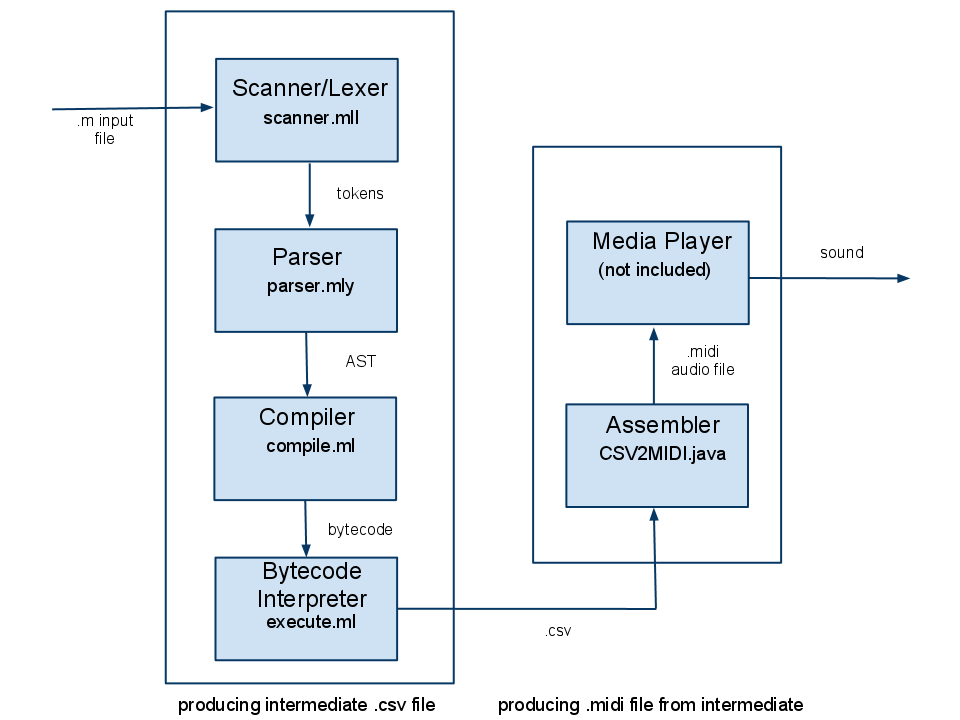
\includegraphics[width=\textwidth]{blockdiagram.png}

\section{Interface between components}
% TODO the reference is broken
The input is a .m file written according to the LRM and the diagram in figure \ref{fig:block_diagram}. The input file is converted into tokens by the scanner/lexer, parsed into an abstract syntax tree, compiled into bytecode, and is further compiled into a CSV by the bytecode interpreter. Finally, the CSV file is assembled into a MIDI file by the Java-based assembler, which can then be played on any standard media player.  The two outputs generated by each .m source file is a .csv file containing CSV information, and a .midi file to be played.  All components are written in OCAML except for the assembler, which is written in Java.  The parser is generated by OCAMLYACC.  The media player is not included here and can be written in any language.

The MIDILC language logically consists of a lexer, parser, bytecode compiler, and assembler.  As the lexer reads in tokens, it invokes the parser.  At this point, syntax errors prevent the compiler from running and output an error.  When parsing is finished, the bytecode compiler is invoked, which generates a series of human-readable CSV bytecodes, which mimic the MIDI structure.  It is at this point that runtime errors (such as granularity issues or bounds check violation) are generated.  Finally, the assembler is run on the CSV to output a type Standard MIDI File.
\section{Who Implemented What}
Fred, Akiva, and Ben: Lexer, Parser, Bytecode, Executor, Compiler

\noindent Fred and Ye: Assembler
\chapter{Test Plan}
\section{Representative Source}
\subsection{For Loop}
\subsubsection{Source Code}
\begin{verbatim}
main() {
  Note a; 
  Sequence b;
  Number i;
  b = new_sequence();
  a = Aq;
  for (i = 0 ; i < 12 ; i = i + 1) {
    b = b + a;
    b = b + ((a as Chord) + (a .+ i));
  }
  play(b);
}
\end{verbatim}
\subsubsection{Bytecode}
\begin{verbatim}
0 global variables
0 Jsr 2
1 Hlt
2 Ent 3
3 Jsr -3
4 Sfp 2
5 Drp
6 Not (69,4)
7 Sfp 1
8 Drp
9 Num 0
10 Sfp 3
11 Drp
12 Sjp (15,23,0)
13 Bra 21
14 Lfp 2
15 Lfp 1
16 Add
17 Sfp 2
18 Drp
19 Lfp 2
20 Lfp 1
21 Cst Chord
22 Lfp 1
23 Lfp 3
24 Dad
25 Add
26 Add
27 Sfp 2
28 Drp
29 Lfp 3
30 Num 1
31 Add
32 Sfp 3
33 Drp
34 Lfp 3
35 Num 12
36 Lt
37 Bne -23
38 Sjp (0,0,3)
39 Lfp 2
40 Jsr -1
41 Drp
42 Num 0
43 Rts 0
\end{verbatim}
\subsubsection{CSV}
\begin{verbatim}
0,4,69
4,4,69
4,4,69
8,4,69
12,4,69
12,4,70
16,4,69
20,4,69
20,4,71
24,4,69
28,4,69
28,4,72
32,4,69
36,4,69
36,4,73
40,4,69
44,4,69
44,4,74
48,4,69
52,4,69
52,4,75
56,4,69
60,4,69
60,4,76
64,4,69
68,4,69
68,4,77
72,4,69
76,4,69
76,4,78
80,4,69
84,4,69
84,4,79
88,4,69
92,4,69
92,4,80
\end{verbatim}
\subsection{Set Instrument}
\subsubsection{Source code}
\begin{verbatim}
main() {
  Note a;
  Sequence b;
  Chord c;
  b = new_sequence();
  a = A3q;
  a = (a as Chord) + C3q + Eb3q;
  b = b + a + a + a;
  set_instrument("Piano");
  play(b);
}
\end{verbatim}
\subsubsection{Bytecode}
\begin{verbatim}
0 global variables
0 Jsr 2
1 Hlt
2 Ent 3
3 Jsr -3
4 Sfp 2
5 Drp
6 Not (57,4)
7 Sfp 1
8 Drp
9 Lfp 1
10 Cst Chord
11 Not (48,4)
12 Add
13 Not (51,4)
14 Add
15 Sfp 1
16 Drp
17 Lfp 2
18 Lfp 1
19 Add
20 Lfp 1
21 Add
22 Lfp 1
23 Add
24 Sfp 2
25 Drp
26 Stn Piano
27 Jsr -6
28 Drp
29 Lfp 2
30 Jsr -1
31 Drp
32 Num 0
33 Rts 0
\end{verbatim}
\subsubsection{CSV}
\begin{verbatim}
0,4,57
0,4,48
0,4,51
4,4,57
4,4,48
4,4,51
8,4,57
8,4,48
8,4,51
\end{verbatim}
\subsection{Arpeggiate}
\subsubsection{Source Code}
\begin{verbatim}
main(){
  Note a;
  Chord c;
  Sequence s;
  Number i;
  
  c = new_chord(C,E,G);
  s = arpeggiate(c);
  play(s);
}

arpeggiate(c)
{
    Number n;
	Number i;
	Sequence s;
	s = new_sequence();
	n = c.length;
	for(i = 0; i < n; i=i+1)
	{
		s = s + c[i];
	}
	return s;
}
\end{verbatim}
\subsubsection{Bytecode}
\begin{verbatim}
0 global variables
0 Jsr 36
1 Hlt
2 Ent 3
3 Jsr -3
4 Sfp 3
5 Drp
6 Lfp -2
7 Mem length
8 Sfp 1
9 Drp
10 Num 0
11 Sfp 2
12 Drp
13 Sjp (7,15,0)
14 Bra 13
15 Lfp 3
16 Lfp 2
17 Lfp -2
18 Ele
19 Add
20 Sfp 3
21 Drp
22 Lfp 2
23 Num 1
24 Add
25 Sfp 2
26 Drp
27 Lfp 2
28 Lfp 1
29 Lt
30 Bne -15
31 Sjp (0,0,3)
32 Lfp 3
33 Rts 1
34 Num 0
35 Rts 1
36 Ent 4
37 Not (67,4)
38 Not (64,4)
39 Not (60,4)
40 Num 3
41 Jsr -4
42 Sfp 2
43 Drp
44 Lfp 2
45 Jsr 2
46 Sfp 3
47 Drp
48 Lfp 3
49 Jsr -1
50 Drp
51 Num 0
52 Rts 0
\end{verbatim}
\subsubsection{CSV}
\begin{verbatim}
0,4,60
4,4,64
8,4,67
\end{verbatim}

\section{Testing automation}
We chose our test cases starting from the most basic, and gradually increased the complexity of them to test and or v.  We initially chose test cases by selecting the basic features of our language (the different data types, basic control features, and built-in functions), and ensuring that they work as expected.  These tests are very simple scripts that include the different ways these language features can be used. For example, we tested the different ways of assigning and modifying Note, Chord, and Sequence types. Test cases that represent previous problem areas, such as the \verb|set_tempo()| function, were chosen next to ensure that these problems have been dealt with.  The next step was to add cases to test all the different ways of modifying data, including use of multiple functions, the dot operator, and the subscript operator.  Some other tests included simple library functions, such as scale generators and major/minor chord generators.  Finally, for completeness, we wrote more complex functions to represent different ways the language would actually be used, including tests that produce full songs and generate harmonies based on melodies.

An automated test suite, based off of the MICROC test suite, was used for regression testing and ensuring that all language features work as expected.  Since our language doesn’t include an interpreter, the interpreter aspect in the MICROC test suite was removed from our test suite. Because our assembler was infrequently modified after the initial implementation, and due to the complexity of assembling each CSV output file, the testing framework compares against the intermediate CSV files instead of the final MIDI output.  Our testing involved running the testall.sh shell script to compare output from each of the tests in the suite, which reports the status for each teset run with either OK or NO (did not pass), before committing any changes.  We did not use a code coverage tool, but instead hand-selected cases that include all aspects of the language, as we believe that this is more well-suited for our language.

Each person performed tests on their own parts of the language. The tests for the features of the complete language, as well as the library functions, were divided among the group. Here is a list of what each member implemented.

\noindent Ben:

	test-add.m
	
	test-chord.m
	
	test-direct1.m
	
	test-divide.m
	
	test-dvorak.m
	
	test-for2.m
	
	test-for3.m
	
	test-note.m
	
	test-rand.m
	
	test-subscript.m


\noindent Fred:

	test-arpeggio.m
	
	test-casts.m
	
	test-chromatic.m
	
	test-chromatic-subscript.m
	
	test-direct.m
	
	test-equality.m
	
	test-gen-harmony.m
	
	test-global.m
	
	test-major.m
	
	test-instrument.m
	
	test-minor.m
	
	test-melody.m
	
	test-numerical-inequality.m
	
	test-shift.m
	
	test-sub.m
	
	test-play-chord.m
	
	test-play-note.m
	
	test-sequence.m
	
	test-tempo.m

\noindent Akiva:
	
	pi-symphony.m
	
	test-for1.m
	
	test-for4.m
	
	test-for5.m
	
	test-recursion.m
	
	test-stairway.m
	
\noindent Ye:
	
	test-harmonicminor.m
	
	test-inequality.m
	
	test-majorscale.m
	
	test-melodicminor.m
	
	test-multiply.m
	
	test-naturalminor.m

\chapter{Lessons Learned}
\section{Most Important Lessons}
\subsection{Akiva Bamberger}
\subsection{Ben Mann}
\subsection{Fred Lowenthal}
\subsection{Ye Liu}
\section{Advice for Future Teams}
\chapter{Appendix}
\end{document}
